\chapter{Background}
\label{sec:background}

This chapter introduces motorsport racing and a number of related concepts that are essential in gaining an understanding of this work. The chapter opens with a brief overview of the sport, followed by an exposition of important concepts like the \emph{racing line}, cornering and braking. A discussion ensues, wherein \emph{understeer} and \emph{oversteer} and explained. A short overview of telemetry is then provided. The chapter concludes with a general introduction to simulation racing rigs.

\section{Motorsport Racing}
In sports, individuals or groups compete to be the first to achieve a particular objective. In circuit motorsport racing, motorised vehicles go round a course for a set number of times. There are varies racing disciplines or series, each one having its own specific rules. However, at the core, participants in all disciplines aim to complete a full lap of the circuit in the shortest time. Some disciplines focus on achieving one fast lap, such as time trials, while others focus on achieving the least amount of time across a fixed number of laps, such as FIA's Formula 1 series. This dissertation will focus on one such discipline, that of confined car racing, which takes place on smooth asphalt surfaces in purpose-built race tracks. 

\begin{figure}[!htb]
	\centering
	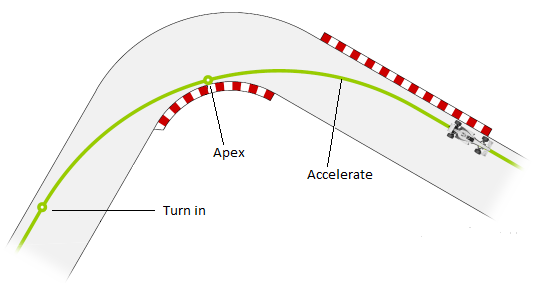
\includegraphics[height=7cm]{images/cornerraceline}
	\caption{Example of confined car racing circuit}
	\label{fig:circuit-overhead}
\end{figure}

\begin{figure}[!htb]
	\centering
	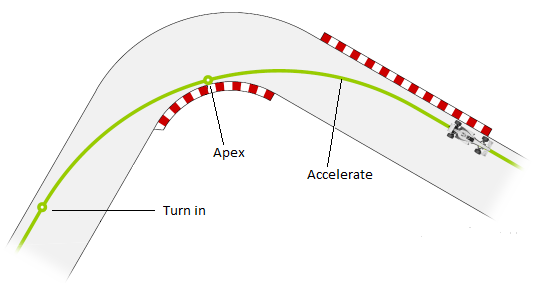
\includegraphics[height=7cm]{images/cornerraceline}
	\caption{Example of racing line, straight and corners}
	\label{fig:circuit-breakdown}
\end{figure}

\begin{figure}[!htb]
	\centering
	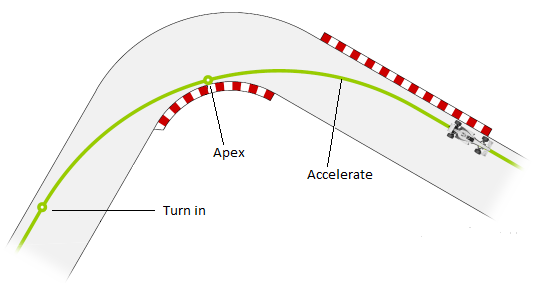
\includegraphics[height=7cm]{images/cornerraceline}
	\caption{Forces acting on a car}
	\label{fig:forces-car}
\end{figure}

\textbf{Figures: Circuit overhead, Racing line overhead, Segmented by straight and corner}

\subsection{Racing Line}
A race driver needs to figure out how to achieve the shortest lap time for a given track.
\emph{A race driver needs to figure out how to go round a piece of asphalt in the minimum amount of time} \cite{GoingFaster}. In order to do so, he or she needs to develop techniques for more advanced vehicle control. One such technique is that of mastering the racing line (see Figure \ref{fig:circuit-breakdown}), which is considered the fundamental skill a race driver must understand and master before moving on to anything else \cite{GoingFaster}. The racing line is the best path through a circuit: if followed, it is the path that yields the shortest time at the highest average speed \cite{beckman1991physics}. The trickiest part of the racing line to master is that which overlaps circuit corner segments (see Figure \ref{fig:circuit-breakdown}). There are two aspects to mastery of the racing line: first, one has to identifying the path which should be taken, and secondly, one must stay on that path. In the first instance, one has to be able to visualise the racing line, while in the latter one has to control the car such that it stays on the line whilst achieving the highest possible average speed. Once the driver can visualise the racing line, he must further partition it, at and near a corner, in three sections. The first section is the breaking part, where the car needs to sufficiently decelerate in preparation for the corner. Braking is usually carried out in a straight line, ending right before the \emph{turn-in point}. The turn-in point refers to a point on the racing line where steering input is applied, forcing the car to turn into the corner. This action should be carried out smoothly, without jerking motions, taking the car all through the corner without too much correction to the steering. Smooth cornering prevents any abrupt changes to the g-forces and centre of gravity of the car (see Figure \ref{fig:forces-car}), which would result in unpredictable car behaviour \cite{GoingFaster}. Thus, the second partition of the racing line at a corner is the segment between the turn-in point and the apex point, which is the inside mid-point of the corner (see Figure \ref{fig:CornerRaceLine}). After the turn-in point, the driver aims for the apex point. The final section of the racing line in a corner lies from the apex point onwards, where the driver must gradually accelerate out of the corner, while still turning, aiming for the outside apex (see Figure \ref{fig:to add}.

\begin{figure}[!htb]
	\centering
	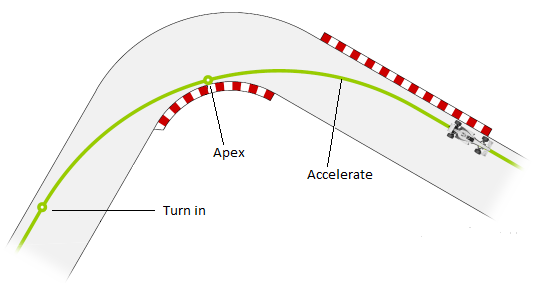
\includegraphics[height=7cm]{images/cornerraceline}
	\caption{Racing line through a 90" right corner}
	\label{fig:CornerRaceLine}
\end{figure}

As the driver gets acquainted to the racing line, usually at sub-optimal speeds, he must find the limit of the car, which is the highest speed the car can be driven while still retaining some measure of control. Various studies have been carried out to define such a limit in terms of the physical properties of the car and its environment \cite{beckman1991physics}. The most important property is the level of grip the car can achieve and sustain on track. A number of factors contribute to the level of grip. Most notably, one very important factor is the tyres as they are the only contact the car makes with the track, and allow for braking, accelerating and turning forces to be transferred to the asphalt. 

Each tyre has two properties which are of particular interest: the slip angle and slip ratio (see Figure \ref{fig:slipangle}). The slip angle is the angle between the tyre's desired direction (perpendicular to the axis of rotation of the tyre) and the tyre's actual direction (the direction the car is moving in). Given both the actual direction of travel ($\mathbf{d}_t$) and the desired direction ($\mathbf{d}_d$) are known, the slip angle $s_a$ is calculated as follows:
\begin{equation}
	s_a = \cos^{-1}(\hat{\mathbf{d}}_d \cdot \hat{\mathbf{d}_t}),
\end{equation}
\noindent where $\hat{\mathbf{d}_d} = \frac{\mathbf{d}_d}{|\mathbf{d}_d|}$ and $\hat{\mathbf{d}_t} = \frac{\mathbf{d}_t}{|\mathbf{d}_t|}$ are the normalised direction vectors for desired and travel directions respectively.

\begin{figure}[!htb]
	\centering
	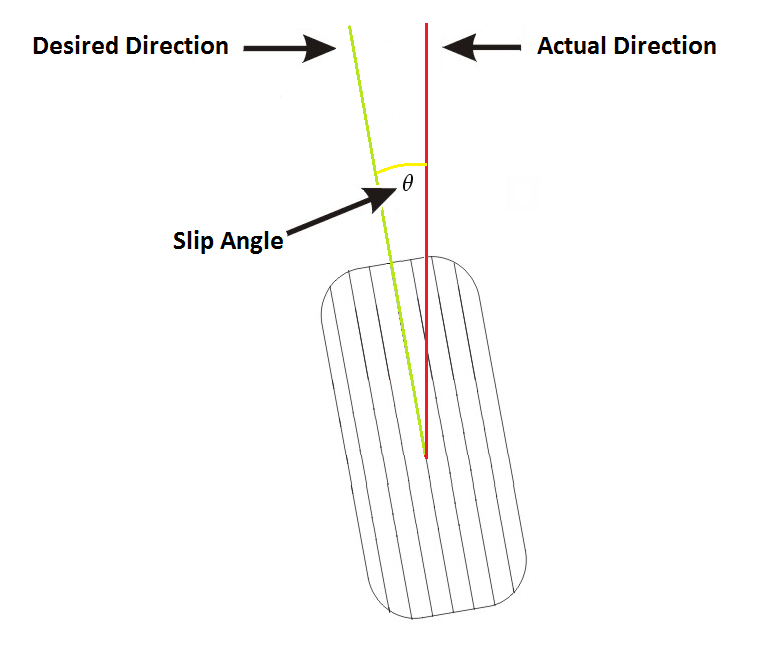
\includegraphics[height=7cm]{images/slipangle}
	\caption{Slip Angle of a tyre understeering while turning left}
	\label{fig:slipangle}
\end{figure}

\subsection{Cornering and Braking}
Whenever the slip angle is above $0\degree$ ($s_a > 0$) the tyre is said to be in an understeering situation. Symptoms include reduced friction, drifting towards the outside of a bend and possible tyre noise from the wheels. Assuming the tyres are not damaged and the track is neither wet nor dirty, understeer can be caused by active factors such as cornering speed, throttle application, braking, steering inputs and weight transfer. Other passive factors such as weight distribution, drive layout, suspension and chassis setup, tyre type, wear and pressures also affect understeer. An understeer situation may be caused by entering the corner at excessive speed, accelerating too aggressively in the corner, breaking through a corner or making sudden input changes which drastically upset the weight distribution of the car. A tyre has an optimal slip angle at which grip is maximised during cornering. The optimal slip angle for a road tyre is about $5\degree$, whereas for a slick tyre, which is purposely constructed for racing, is about $8\degree-10\degree$ \cite{beckman1991physics}.

%Passive factors have to do with the way a car is mechanically setup, such factors will be taken in consideration during this project but will not be given great importance as this project aims to improve the drive’s skills. The project will focus on the active factors as these are the ones which the driver has direct input on while driving a car. 

An oversteering situation may arise from lack of grip; while understeer is caused by a lack of grip in the front tyres, oversteer is cause by a lack of grip on the rear tyres. Oversteer is usually denoted by the rear of the vehicle becoming unstable resulting in its rotation such that the driver is facing towards the inside of the corner. Similarly to understeer, the active factors causing oversteer are also cornering speed, throttle application, braking, steering inputs and weight transfer. Oversteer is usually induced by braking during a corner or accelerating too hard in a rear wheel drive vehicle.
%
%Active factors causing oversteer are cornering speed, throttle, braking, steering inputs and weight transfer. The driver can avoid oversteer by not braking while in a corner and not accelerating too hard in a rear wheel drive as it makes the rear tyres spin too fast, losing traction with the road.

\begin{figure}[!htb]
	\centering
	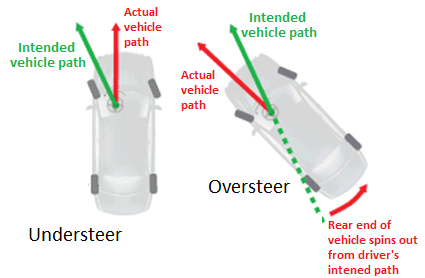
\includegraphics[height=7cm]{images/overundersteer}
	\caption{Visual representation for oversteer and understeer}
	\label{fig:slipangle}
\end{figure}

During acceleration and braking the tyre experiences rotational forces; when these rotational forces do not match the expected velocity, there is some level of slip occurring between the tyre and the road. This is referred to as \emph{slip ratio} and is expressed as a percentage: a slip percentage of 100\% means that the tyre is rotating but the road is stationary. In jargon, this is called \emph{burnout} or \emph{wheel spin}. On the other hand, a percentage of -100\% indicates that the tyre is not rotating but the road beneath is moving. This can occur when braking too hard and is called \emph{locking the wheels} \cite{pacejka2006tire}. While braking the driver must avoid locking up the tyres as this will cause them to wear out more quickly, while drastically increasing the stopping distance. Conversely, braking too lightly makes the car decelerate at a slower rate, losing the driver precious time. For an optimal braking procedure, the slip ratio should be between 10\% to 15\% \cite{GoingFaster}.

Passive factors, which depend on the mechanical set up of a car, may also influence car behaviour during cornering and braking. However, in this work, any passive factors will be normalised and kept constant across all the study to eliminate any possible effects on dependent variables. 

\subsection{Telemetry Data}
Telemetry (literally remote measurement), is the automated communications process by which measurements and other data are acquired from remote or inaccessible objects or sites, to be subsequently monitored \cite{nasaTelemetry}. Telemetry data is domain specialised data that contains such measurements, transmitted to receiving equipment for remote monitoring. In motorsport, telemetry data contains measurements of vehicle dynamics from the engine and other components. These measurements can serve to monitor and reconstruct the vehicle state at a particular point in time. Telemetry data in motorsports usually accounts for measurements of speed, engine speed, component temperatures, slip angles, slip ratios, etc. Telemetry is widely regarded as the most important source of information by motorsports engineers; analysing this data can lead to a better understanding of the respective strengths and weaknesses of the car and the driver \cite{CarDataAnalysis}. In this work, we posit that through the real-time analysis of telemetry data, the pedagogical aspect of sim racing can be exploited to teach race driving to non experts.  

\begin{figure}[!htb]
	\centering
	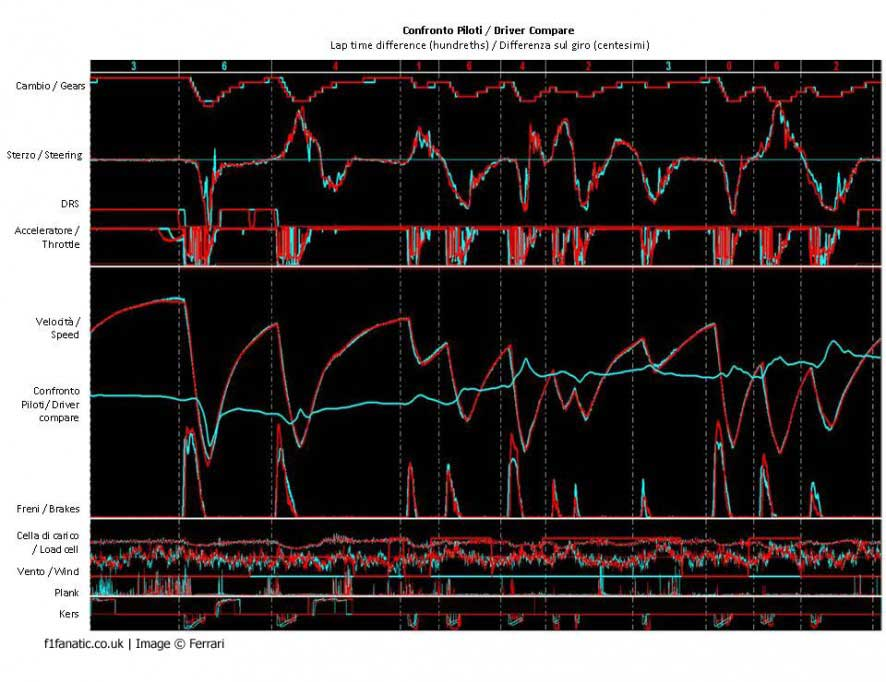
\includegraphics[height=7cm]{charts/telemetrydata.jpg}
	\caption{Visualisation of racing car telemetry data}
	\label{fig:telemetrydata}
\end{figure}

\section{Racing Simulation Rigs}
The racing simulation rig (sim racing rig) is a piece of equipment designed to mimic the cockpit of a real-world car. The quality of a sim racing rig is dependent on its authenticity - how similar it is to a real-world car - and its build quality. These rigs come in various shapes, forms and sizes, from hangar-sized hydraulic-driven car chassis, that cost millions of Euro, to the more modest, built from off-the-shelf commodity hardware. Minimally, a rig should provide a steering wheel, seating and a display. More sophisticated rigs augment the user experience by employing gear shifters, and clutch, throttle and breaking pedals. The more advanced components are furnished with a force feedback mechanism, a form of haptic technology used to replicate the sense of touch by applying forces or vibrations, or motions to the user \cite{li2015can}. Force feedback may be caused by electrical motors, gear trains or hydraulic systems. In high-end rigs, for instance, hydraulic systems are used to simulate the latitudinal and longitudinal forces to which a driver is exposed during driving. Modern rigs might include virtual reality headsets as a replacement for displays, to enhance immersion and increase realism.

\begin{figure}[!htb]
	\centering
	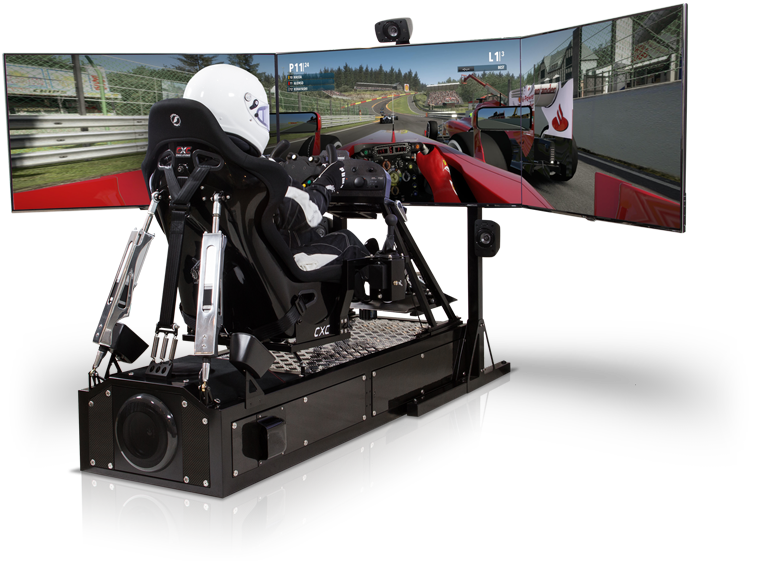
\includegraphics[height=7cm]{images/proracingrig.png}
	\caption{Professional racing rig by CXC Simulations}
	\label{fig:slipangle}
\end{figure}

\section{Summary}






